\documentclass{article}

% Language setting
% Replace `english' with e.g. `spanish' to change the document language
\usepackage[english]{babel}

% Set page size and margins
% Replace `letterpaper' with `a4paper' for UK/EU standard size
\usepackage[letterpaper,top=2cm,bottom=2cm,left=3cm,right=3cm,marginparwidth=1.75cm]{geometry}

% Useful packages
\usepackage{amsmath}
\usepackage{graphicx}
\usepackage[colorlinks=true, allcolors=blue]{hyperref}

\title{Protein Structures}
\author{Vinay Kakkar}

\begin{document}
\maketitle

\begin{abstract}
Abstract here!
What the report is about
Short part to explain why we need this report
\end{abstract}

\section{Introduction}

Proteins are responsible of catalysing almost all the chemical reactions in the cell. Proteins can function as enzymes catalysing a wide variety of reactions necessary for life and they can be important for the structure of living systems such as those proteins involved in the cytoskeleton. The size of protein can vary from small to quite large macromolecules.

Catalysing: cause or accelerate (a reaction) by acting as a catalyst.
Cytoskeleton: dynamic network of interlinking protein filaments present in the cytoplasm of all cells

DNA sequence of gene can be analysed to give the amino acid sequence of the protein product. Bioinformatics uses this knowledge that can help deduce the likely properties of unknown proteins, plus their functions and structures. Knowing the relationship between a proteins structure and its function provides a greater understanding of how the protein works and thus enables the researcher to propose experiments to explore how modifying the structure will affect the function. Interacting with proteins, structure-function studies are vital to the design of new drugs and bioinformatics speeds this up and provides computer modelling of these interactions.


\section{Protein Structure}

\subsection{Primary and Secondary Structure}

\subsubsection{Protein structure can be considered on several different levels}

A protein folds into a three-dimensional structure, which is determined by its protein sequence. The fold of the protein consists of repeating structural units called secondary structures. The fold of the protein is very important for the way the protein will function, and whether it will function correctly. Therefore the study of the ways in which proteins fold and understanding how they fold is an important area of bioinfor- matics, as well as predicting the fold of a protein from its sequence.

Protein structure can be considered on several different levels
The analysis of protein structure by experimental techniques such as X-ray crystal- lography and nuclear magnetic resonance (NMR) has shown that proteins adopt distinct structural elements. The primary structure is the protein sequence, the types and order of the amino acids in the protein chain. the secondary structure is the first level of protein folding, in which parts of the chain fold to form generic structures that are found in all proteins. The tertiary structure is formed by the further folding and packing together of these elements to give the final three-dimensional conformation unique to the protein. Many functional proteins are formed of more than one protein chain, in which case the individual chains are called protein subunits. The subunit composition and arrangement in such multisubunit proteins is called the quaternary conformation. The structure adopted by a protein chain, and thus its function, is determined entirely by its amino acid sequence, but the rules that govern how a protein chain of a given sequence folds up are not yet understood and it is impossible to predict the folded structure of a protein de novo from its amino acid sequence alone. Helping to solve this problem is one of the challenges facing bioinformatics.

De novo: he first occurrence of cancer in the body

\begin{figure}
    \centering
    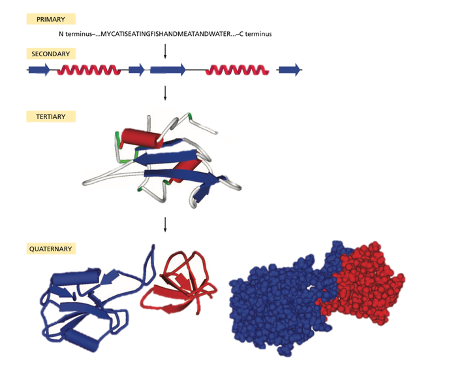
\includegraphics[width=0.5\textwidth]{Protein Structure.png}
    \caption{\label{fig:Simple schematic showing the different levels of protein structure.}From the sequence alone (the primary structure) to secondary structure (which contains local structural elements), to tertiary structure (where the structural elements fold to give a three-dimensional structure), to finally quaternary structure found when several tertiary structures form a multisubunit complex.}
\end{figure}

Amino acids are the building blocks of proteins
Proteins are made up of 20 types of naturally occurring amino acids with a few other amino acids occurring infrequently. of an amino acid can be divided into a common main chain part and a side chain that differs in chemical structure among the different amino acids. The side chain is attached to the main chain carbon atom known as the a-carbon.

The differing chemical and physical properties of amino acids are due to their side chains
The functional properties of proteins are almost entirely due to the side chains of the amino acids. Each type of amino acid has specific chemical physical properties that are conferred on it by the structure and chemical properties of its side chain. They can, however, be classified into overlapping groups that share some common physical and chemical properties, such as size and electrical charge. Some side chains can be charged and not charged they can even be negatively or positively charged. 

Amino acids are covalently linked together in the protein chain by peptide bonds
The primary structure of a protein is the sequence of amino acids in the linear protein chain, which consists of covalently linked amino acids. This linear chain is often called a polypeptide chain.

\begin{figure}
    \centering
    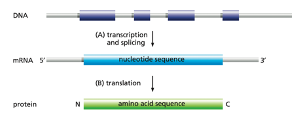
\includegraphics[width=0.5\textwidth]{Transcription and translation.png}
    \caption{\label{fig:Transcription and translation}The relation of DNA coding-strand sequence to mRNA sequence to protein sequence. The exons (purple boxes) of the DNA are transcribed into mRNA which, using other molecules directs the protein sequence.}
\end{figure}

Secondary structure of proteins is made up of a-helices and b-strands
It should be noted that the structures found in globular proteins are not perfectly regular, so it is frequently difficult to define the precise ends of the helices, and in some cases the hydrogen-bonding patterns are intermediate between these idealized forms. Therefore, prediction of these structures using bioinformatics programs is made more difficult.

Several different types of b-sheet are found in protein structures


Turns, hairpins, and loops connect helices and strands
Any chain between two regular structures is referred to as a loop. In many cases a loop will contain a turn (or even several). In general there are no classifications for loops, but there is an important exception. In antibody recognition, immunoglobulins employ loops at the edge of a b-sheet to recognize the antigen. There are vast numbers of different immunoglobulin structures, all with the same overall chain fold, but it is the difference at these loops that results in different affinities. With many structures known, it has been observed that the loops take up one of a limited number of structures (called canonical forms), so that in this particular case the loops have been classified. This type of classification is important when trying to predict both the structure and function of the protein.


\subsection{Proteins Fold to Form Compact Structures}

Protein chains themselves rarely have any biological function. Only when the chain has folded up into a three-dimensional structure (however small) does the protein have functional activity. Some proteins are enzymes that bind other molecules (ligands) and catalyze their biochemical reactions, others act by binding other proteins and influencing their activity, and yet others bind to DNA and regulate gene expression. Some proteins have a purely structural function, making up the fabric of the cell. Large numbers of proteins are released, or secreted, from cells and act as chemical messengers, influencing the behavior of other cells by acting on yet another large functional class of proteins, known as receptors, on cell surfaces.

The tertiary structure of a protein is defined by the path of the polypeptide chain
In the tertiary structure of a protein, various combinations of secondary structure pack together to form a compactly folded mass. In a multidomain protein it is thought that each domain folds independently of the others. Bioinformatics questions are often concerned with comparing the sequences and structures of different domains rather than whole proteins. A domain can be anything from 50 to around 350 amino acids in length. The core of each domain is mainly composed of tightly packed a-helices, b-sheets, or a mixture of both. The three- dimensional structure of a protein is known as its conformation. More specifically, the spatial path of any given folded polypeptide chain is known as its fold.

As proteins exist in an aqueous environment, folding tends to result in hydrophobic regions of the protein ending up in the interior, while more hydrophilic regions are on the outside. A variety of noncovalent interactions stabilize the fold, dominated by hydrogen bonding and the clustering of hydrophobic groups. Secondary structures pack together in a variety of ways, such as the formation of b-sheets from either parallel or antiparallel b-strands. The atoms pack together very efficiently in most natural proteins.

There appears to be a limited number of ways in which secondary structures fold into domains. There are several instances where proteins that seem to be completely unrelated in terms of sequence are found to have the same fold and some researchers estimate that there may be only a few thousand different folds in nature. Currently, there are more than 35,000 known protein structures, and these are classified into approximately 2000 fold families. The fact that so many proteins fold into a similar structure even if their sequences are not very similar means that we can use bioinformatics tools to model structures of various proteins on similar folds

The stable folded state of a protein represents a state of low energy
A protein chain starts to fold as soon as it has been synthesized and thermodynamic considerations mean that the final fold it adopts is a state of low free energy. Folded proteins are generally stable in the conditions in which they have to operate, but in a wider sense, proteins are unstable thermodynamically. Most proteins start to unfold above about 60∞C, as the noncovalent bonds that hold them together are broken by thermal energy; unfolded proteins are said to be denatured. As it becomes denatured, a protein loses its function. Only specialized microorganisms are capable of living at temperatures this high.


Many proteins are formed of multiple subunits
Individual folded polypeptides can interact with each other to form protein complexes or quaternary structures.


\section{Large Scale Experssion}

\subsection{Large Scale Gene Expression}

\subsection{Large Scale Protein Expression}

\section{Alpha Fold}

Alpha Fold

\section{Implication for Bioinformatics}

In part, bioinformatics concerns itself with the analysis of protein sequence to predict the secondary structure, the tertiary structure, and the function of the protein, as well as its relationship to other proteins. Different secondary structures tend to have subtle differences in chemical environments, resulting in amino acid preferences. In addition, amino acid preferences are seen at particular locations in proteins due to the functional role they play, for example as catalytic residues or stabilizing the overall protein structure.


Certain amino acids prefer a particular structural unit
Due to the various properties of the amino acid side chains, certain residues or certain types are found more often in one or the other of the structural units.


Evolution has aided sequence analysis
Protein sequence similarity is a powerful tool for characterizing protein function and structure since an enormous amount of information is conserved throughout the evolutionary process. Sequence alignment and database search techniques can identify homologous proteins. Homologous proteins usually have a similar three-dimensional structure with related active sites and binding domains. Therefore homologous proteins will also often have related functions, although this is not always the case. Most amino acids that change during evolution are found in regions that are not structurally or functionally important, such as many of the loops (or variable) regions. f the homologous protein is also functionally related then the amino acids involved in function are often conserved during evolution, which helps in identifying the function of a new protein

Homologous: Proteins that have a common ancestor 
Visualization and computer manipulation of protein structures
There are a number of programs available that read the coordinate file and convert it to a visible three-dimensional representation of the protein. The protein can be rotated, specific regions highlighted, and some measurements can be calculated. Some of these programs are very powerful and can be of great use in analyzing the structural properties and molecular function, as well as allowing for the manual modification of the molecule. Some of the programs are free or low cost, such as Chimera, Yasara, and DeepView. Others are extremely powerful programs that allow the user to carry out computationally intensive modifications to the molecule, but are expensive.


\bibliographystyle{alpha}
\bibliography{sample}

\end{document}